\documentclass{article}

\usepackage{graphicx}
\usepackage{verbatim}

\begin{document}

\section{Parallellizing the thickness algorithm}

\noindent 1) Explain Thickness of Knot

\noindent 2) Explain Thickness Algo

Now we would like to compute the thickness in parallel using
more than a single CPU. This is natural since the bisections
are done on a per arc pair basis. Once we have a set of candidate
arc pairs the only remaining thing to do is computing the minimal
distance on arcs containing a double critical point. The smallest
of these values is the thickness of the knot.

Every child process gets a few candidate
arc pairs and computes the minimal distance on double critical
arcs, if it exists. The master handles in a client server way
the communication with the child processes by sending new arc
pairs and the currently best thickness value. If a child reports
to be done with its work it sends back the distance found. If the
computed distance is either larger than the one received from
the master or there are no double critical points found, then the
distance value send back to the master is simply a large number.

In what follows we'll discuss the tasks for master and child processes,
present the details of the complete algorithm, go into implementation
issues and present some benchmark results. The last part points out
possible improvements.

\subsection{Client/server, master/children}

The master or root process initializes the knot and computes a first
set of candidate arc pairs. Now it has to send one or more pairs to
every available child, which will compute the shortest distance on the
pairs. Once every child has gotten its first workload, the master cycles through
them and waits for children done with their task. The child reports back
the computed distance and the master immediatly sends the next arc pair (or more
than one) to constantly keep the children busy. Every time the master
receives a distance value from a child, it updates the thickness
and sends this value in future jobs. As soon as all the arc pairs are processed,
the master notifies the child processes that their work is done and
ends.

\begin{comment}
\begin{figure}[p]
\includegraphics[width=\textwidth]{parallel_algo_flowchart.pdf}
\caption{XXX Explain chart! \label{fig:parallel_algo_flowchart} }
\end{figure}
\end{comment}

\subsection{MPI: A Message-Passing Interface Standard}

The MPI API specification is a standart for MIMD parallel computing
that defines how different processes with separate memory spaces
communicate to fullfill a computation or program execution. The
communication is done with a message passing protocol between the
various processes running in parallel. The communication between
processes can be point-to-point (blocking) or asynchronous (non-blocking).
A point-to-point communication is considered to be finished when
the sender and receiver exchanged the data. For the non-blocking
case the sender does not wait until the data has been received
by its communication partner.

Different computer and cluster manifacturers have different
implementations of the MPI interface tailored to their hardware.
A relatively widespread implementation is MPICH, which has
as well been used as a bases for MPI implementations.
LAM or openMPI are other implementations of this interface standard.

We will not present the entire list of MPI functions. As an example
we start with a minimal program.

\begin{verbatim}
#include <stdio.h>
#include <mpi.h>

int main (int argc, char *argv[]) {
  int rank, size, 

  MPI_Init(&argc, &argv);

  MPI_Comm_rank(MPI_COMM_WORLD, &rank);
  MPI_Comm_size(MPI_COMM_WORLD, &size);

  printf("Process %d of %d\n", rank, size );

  MPI_Finalize();

  return 0;
}
\end{verbatim}

In the program listing we use \verb+MPI_Init+ to intialize
the MPI environment and \verb+MPI_Finalize+ to end the
execution. The function \verb+MPI_Comm_rank+ asks what
processor number this process has and
\verb+MPI_Comm_size+ requests information about how many
CPUs are available. 

Running MPI programs in a parallel environment such as
a computing cluster depend on the different implementations.
A sample invocation using $4$ CPUs would be the following

\begin{verbatim}
mpirun -machinefile machines -np 4 program
\end{verbatim}

where the file \verb+machines+ contains information about
the cluster like node hostnames and number of processors per
host.

Two other routines are worth mentioning since they are
the basis of every parallel program for sending and
receiving messages.

\begin{verbatim}
int MPI_Send( void *buf, int count, MPI_Datatype datatype, int dest, 
              int tag, MPI_Comm comm )
int MPI_Recv( void *buf, int count, MPI_Datatype datatype, int source, 
              int tag, MPI_Comm comm, MPI_Status *status )
\end{verbatim}

The various arguments are \verb+buf+, a pointer to the data to be
sent or received - \verb+count+, the size of the data of type
\verb+datatype+. The integers \verb+dest+ and \verb+source+ define
the rank of the partner process, \verb+tag+ is a message identification
and \verb+MPI_Comm+ is a communication handle. A common handle is
\verb+MPI_COMM_WORLD+ which includes all the available processes.
It is possible to define other communicators depending on the
network and computation topology implemented in the program.

Collective communication is possible as well. A broadcast sends
a message to all the processes, scatter and reduce sends one task
to all the processes in a group or reduces values on all processes to a
single value on one process.

\subsection{Custom datatypes}

The MPI standard defines a series of datatypes like \verb+MPI_INT+ or
\verb+MPI_DOUBLE+. In this algorithm we have to send information concerning
the candidate arc pairs to the computing children. Every message passed from one
process to another must have a specified datatype. We want to send a message
containing enough information for the child processes to be able to compute the
minimal distance. That's why a new MPI datatype was necessary. It is possible
to define an entire structure as a new MPI datatype, which in our case would be
the \verb+Candi<Vector>+ class. However, the size of this structure is $248$ bytes,
which would cause considerable communication overhead. In order to compute the
minimal distance we only need the bezier points ($9+9$ double) for the arc pair,
error information ($2+2$ double) associated with each arc and the currently best
minimal distance ($1$ double) for the subdivision process. This is a total of $23$
doubles adding up to $184$ bytes, which is better than sending the whole struct.
We add one more double used as signal. Implementing signals floating point values
is usually a bad idea due to rounding errors, but here we set this value larger
than $0$ if we want the receiving process to compute the distance and smaller than
$0$ if we want to inform the process that it can exit. An alternative could be a
MPI mixed data type, where we would use a single bit as a signal and the $23$ doubles.
The implementation is easier with only doubles and with a single bit alignement
problems could occur due to fixed buffer lengths in the sending and receiving process.

The new datatype is therefore an array of $24$ doubles, initialized at the beginning
of the MPI program with

\begin{verbatim}
MPI_Datatype MPI_Candi;
MPI_Type_contiguous(24, MPI_DOUBLE, &MPI_Candi);
MPI_Type_commit(&MPI_Candi);
\end{verbatim}

This datatype can then be used just like \verb+MPI_INT+ or \verb+MPI_DOUBLE+.
The next thing to do is prepare the data to be sent to the child processes.
For that purpose we have the two following two routines

\begin{verbatim}
void pack_candidate(const Candi<Vector3> &c, const double curr_min, double res[24]);
void unpack_candidate(const double res[24], Candi<Vector3>* c, double *curr_min);
\end{verbatim}

The function \verb+pack_candidate+ fills an array of doubles with the information
needed from \verb+Candi<Vector3>+ and \verb+unpack_candidate+ initializes the
\verb+Candi<Vector3>+ from \verb+res+. Since the master process has a list
of candidates to process, it packs the data in an array of doubles and sends it to
the child process, which then unpacks it into a \verb+Candi<Vector3>+ object.
The minimal distance gets computed and only this double value is sent back to
the master.

\subsection{Batching candidates}

Subdivision on one arc pair can finish very quickly depending on how close
we alredy are to the final thickness value. The consequence is that the child
processes will ask for new candidate pairs and the master might become a bottleneck
if he's only busy sending out new candidates to the children. To reduce this
communication overhead we can play with the number of arc pairs we send at once.
This is called batching and needs more memory to store all the arc pairs, but then
the children simply process the whole list and only when finished, they ask for
new pairs. This is implemented like

\begin{verbatim}
MPI_Send(serial, BATCH, MPI_Candi, i, TAG, MPI_COMM_WORLD);
MPI_Recv(serial, BATCH, MPI_Candi, 0, TAG, MPI_COMM_WORLD, &stat);
\end{verbatim}

where \verb+serial+ is the send/receive buffer, \verb+BATCH+ the number of arc
pairs, $i=1,\ldots, \#CPUs-1$ is the child process rank ($0$ for the master). Whether
batching speeds up the computation depends on various parameters like the number
of arc pairs, the knot shape, local curvature active, etc.

\subsection{Code snippets showing the algo implementation}

\subsection{Discussion}

% time vs cpus
In what follows we use an approximately ideal trefoil to test the program. Everything
has been computed on an Intel "Woodcrest" cluster with one master and $14$ bi-dual nodes.
Figure \ref{fig:time_vs_cpus} shows the time needed to compute the thickness in function
of the number of CPUs. Up to $10$ CPUs, the speed improvement can seams reasonnable. For more
than $10$ CPUs the gain flattens out and is no longer useful. The master can no longer
serve the children at full speed, since there are too many, and slows down the whole computation.

% time vs nodes
The next experiment is shown in Figure \ref{fig:time_vs_nodes}, where we vary the number of
knot data points, keeping the number of CPUs at $8$ for all the runs. Compare this to the
standard thickness computation on a single CPU. We can see a more or less linear behaviour with
a slope visibly smaller for the multi CPU case. Parallelization becomes interesting if we
have to compute with extremely refined knot shapes as it is the case at the so called end-game.

% time vs batch size
Earlier we discussed that the master could send more than a single candidate pair to the
child processes. Figure \ref{fig:time_vs_batch} plots the time versus the number of arc
pairs we send in a row. The knot shape has $512$ data points and we vary the batch size
between $1$ and $100$. The computation gets faster the more candidates we send at once.
The resulting communication overhead seems negligeable compared to the speed we win by giving a
lot of work to the child processes. A batch size larger than $100$ slows the computations
down, here is where the communication overhead starts to interfer. The master's minimal distance
value allows us to discard a lot of candidates early on, but this is no longer the case if
we send batches to each child process.

% time vs various knots
Another delicate point is the actual shape. Different shapes might lead to completely different
timings depending on how close various parts are to the final thickness. If a knot has several
"good" regions it will take much longer to converge on a single processor. All the subdivisions
have to be carried out until the relative tolerance is reached and only then can the master
compare the various values and compute the smallest one. sequentially, then . The computations
in Figure \ref{fig:time_vs_knots} show that the speed-up can be significantly different from
one knot shape to another. For the knots where the time of a single CPU comes very close to the $8$
processor run could be explained by this worst case scenario : In parallel we compute $7$ arc pairs
and the master receives $7$ distance answers, where the smallest is used for the next $7$ arc pairs.
If we would follow these $7$ candidates in the single CPU case it might happen, that the first
pair is already the smallest out of the $7$ and the next $6$ are rejected since they can not yield
a lower value. If this is true for almost every block of $7$ pairs, then the times for the single
and multi processor runs have to be close.

\begin{comment}
\begin{figure}
\includegraphics[width=\textwidth]{time_vs_cpus.pdf}
\caption{XXX Explain \label{fig:time_vs_cpus}}
\end{figure}

\begin{figure}
\includegraphics[width=\textwidth]{time_vs_nodes.pdf}
\caption{XXX Explain \label{fig:time_vs_nodes}}
\end{figure}

\begin{figure}
\includegraphics[width=\textwidth]{time_vs_knots.pdf}
\caption{XXX Explain \label{fig:time_vs_knots}}
\end{figure}

\begin{figure}
\includegraphics[width=\textwidth]{time_vs_batch.pdf}
\caption{XXX Explain \label{fig:time_vs_batch}}
\end{figure}
\end{comment}

\subsection{Timing master/slaves}

%We now adress the time for the master and the slaves. 
%XXX Continue, make plots, for trefoil and 3.1 (3.1 master is 50% of total time)

A different analysis, compared to the various parameters discussed above, is
the time the master needs to do the initial setup and preliminary computations.
Table \ref{tab:master_slave_timing} summarizes this for the first knot of every knots
with a number of crossings up to $9$. The knot $j3.1$ has been computed by \cite{XXX}
and is a very good approximation for an ideal trefoil knot. These times indicate,
that the master spends a lot of time at the beginning. For the $k3.1$ the master
needs the same time as the children, for the $k5.1$ the children do basically
nothing compared to the master. On the other side there is the $j3.1$, where
the initialization step takes only a fraction of the afterwards following
computation by the child processes. A more in depth analysis has shown that
the masters spends most of the time to set up the inital candidate arc pairs.
Note that the batch size has been set to $1$ for these computations.

\begin{comment}
\begin{figure}
\begin{center}
\begin{tabular}{lclll}
knot & data points & master (sec) & children (sec) & total (sec) \\
j3.1 & 512 & 0.165336 & 2.092650 & 2.258000 \\
k3.1 & 160 & 0.016368 & 0.016206 & 0.032578 \\
k4.1 & 208 & 0.024819 & 0.018046 & 0.042868 \\
k5.1 & 232 & 0.031302 & 0.000165 & 0.031471 \\
k6.1 & 280 & 0.042829 & 0.000162 & 0.042995 \\
k7.1 & 304 & 0.052276 & 0.013455 & 0.065735 \\
k8.1 & 352 & 0.067262 & 0.012944 & 0.080209 \\
k9.1 & 376 & 0.067325 & 0.000118 & 0.067447
\end{tabular}
\end{center}
\caption{XXX caption \label{tab:master_slave_timing} }
\end{figure}
\end{comment}

\subsection{Possible improvements}

The above analysis of the various parts and parameters of the algorithm
points out a few weak points and ideas for optimizations. The master might
have a lot to do with interprocess communication if the children finish
rapidly their computations, however if this is not the case, then the
master is idel, waiting for child processes to send back their values,
when it could compute as well some candidate pairs. If we make the master
compute as well, then some of the children might have to wait until the
master answers again the phone, waisting precious time. This issue could
be surmounted by implementing an interrupt system, where the children
stop the master in its computation, send the value and receive new pairs.
XXX However we do not know if MPI supports this type of communication.
The master's minimal distance value is important to quickly discard
pairs if they can not achieve better. Keeping the children up to date
by sending them a new distance value whenever the master receives a
better thickness (for example by broadcasting) would deal with that problem. 
Table \ref{tab:master_slave_timing} pointed out that the master
spends a lot of time in the initialization step, mainly by setting up the
arc pairs and the first double critical filter. Delegating part of this
first filtering to the children would reduce the master's work. Considering
the underlying implementation the initial filtering is based on, this
would require quite a few changes.

\end{document}
